\chapter{Complexidade Computacional}
\label{cha:complexidade}

Até aqui nos ocupamos principalmente do problema da expressivdade de modelos de computação.
Ou seja, o que é possível computar com cada modelo.
Terminamos o último capítulo com um modelo bastante expressivo das Máquinas de Turing.
Vimos que mesmo nesse modelo há problemas que não são computáveis, como o problema da parada.

Neste último capítulo nos voltaremos para outra questão: que problemas computacionais são resolvíveis de maneira eficiente?
Por efeciente entendemo que há algum recurso escasso consumido pelo algoritmo que resolve o problema, por exemplo tempo ou espaço de memória.

\section{Complexidade de Tempo}
\label{sec:tempo}

O {\em tempo de execução} de uma MT $M$ é uma função $f: \mathbb{N} \to \mathbb{N}$ em que $f(n)$ é o número máximo de passos de derivação para uma entrada $\omega$ qualquer de tamanho $n$.

\begin{displaymath}
  TIME(t(n)) = \{A \subseteq \Sigma^* : \textrm{$\exists$ MT simples que decide $A$ em tempo $O(t(n))$}\}
\end{displaymath}

\begin{example}
  $TIME(n)$ é a classe dos problemas resolvíveis em tempos {\em linear} no pior caso.

  $TIME(n^2)$ é a classe dos problemas resolvíveis em tempo {\em quadrático} no pior caso.
\end{example}

\begin{theorem}
  Se $t(n) \geq n$ então toda MT multifita que consome tempo $t(n)$ é equivalente a uma MT simples que consome tempo $O(t^2(n))$.
\end{theorem}
\begin{proof}
  Considere a simulação de uma MT com $k$ fitas que vimos no Teorema \ref{}.

  $M$ varre a fita em tempo $O(n)$ para obter as informação necessárias para o próximo passo.

  Para executar um passo $M$ no pior precisamos abrir um espaço em branco na fita e para isso deslocamos todo conteúdo uma posição para a direita.
  Nesse caso como o tamanho máximo da fita é $O(t(n))$, precisaríamos de $O(t(n))$ passos para esse deslocamento.

  Assim, o tempo total de excecução é $t(n).O(t(n)) + O(n)$.
  Se $t(n) \geq n$ então $t(n).O(t(n)) + O(n) = O(t^2(n))$.
\end{proof}

O tempo de execução de uma MT não-determinística $N$ é uma função $f: \mathbb{N} \to \mathbb{N}$ em que $f(n)$ é o número máximo de passos de {\em alguma} derivação de $N$ para a entrada $\omega$ de tamanho $n$.

\begin{multicols}{2}
\centering
Determinístico

\vspace{1cm}

\begin{tikzpicture}[node distance=2cm,auto,>=latex,initial text=]
  \draw [|-|] (-2,0) -- node[left]{$f(n)$} (-2,-8);
  \node[circle, draw] (q0) {};
  \node[circle, draw] (q1) at (0, -2) {};
  \node[circle, draw] (q2) at (0, -4) {};
  \node[circle, draw] (qn) at (0, -8) {};
  \path[->] (q0) edge (q1);
  \path[->] (q1) edge (q2);
  \path[-, dashed] (q2) edge (qn);
\end{tikzpicture}


\columnbreak
\centering
Não Determinístico

\vspace{1cm}

\begin{tikzpicture}[node distance=2cm,auto,>=latex,initial text=]
  \node[circle, draw] (q0) {};
  \node[circle, draw] (q11) at (-2, -2) {};
  \node[circle, draw] (q12) at (0,  -2) {};
  \node[circle, draw] (q13) at (2,  -2) {};
  \node[circle, draw] (q21) at (-4, -4) {};
  \node[circle, draw] (q22) at (-2, -4) {};
  \node[circle, draw] (q23) at (0,  -4) {};
  \node[circle, draw] (q24) at (2,  -4) {};
  \node[circle, draw] (q25) at (4,  -4) {};
  \node[circle, draw] (qn1) at (-4, -8) {};
  \node[circle, draw] (qn2) at (-2, -8) {};
  \node[circle, draw] (qn3) at (0,  -8) {};
  \node[circle, draw] (qn4) at (2,  -8) {};
  \node[circle, draw] (qn5) at (4,  -8) {};
  \path[->] (q0) edge (q11);
  \path[->] (q0) edge (q12);
  \path[->] (q0) edge (q13);
  \path[->] (q11) edge (q21);
  \path[->] (q11) edge (q22);
  \path[->] (q12) edge (q23);
  \path[->] (q13) edge (q24);
  \path[->] (q13) edge (q25);
  \path[-, dashed] (q21) edge (qn1);
  \path[-, dashed] (q22) edge (qn2);
  \path[-, dashed] (q23) edge (qn3);
  \path[-, dashed] (q24) edge (qn4);
  \path[-, dashed] (q25) edge (qn5);
\end{tikzpicture}

\end{multicols}


\begin{theorem}
  Se $t(n) \geq n$ então toda MT não-determinística que consome tempo $t(n)$ é equivalente a uma MT simples que consome tempo $2^{O(t(n))}$.
\end{theorem}
\begin{proof}
  Vimos no Teorema \ref{} como simular uma MT não-determinística $N$ usando uma MT com 3 fitas usando uma busca em largura.

  Seja $b$ o número máximo de ramificações de na excecuçaõ $N$.
  O número total de nós da árvore é $O(b^{t(n)})$ e a excecução de cada nó toma tempo $O(t(n))$ no pior caso.

  Assim, o tempo total de excecução dessa simulação é $O(t(n).b^{t(n)}) = 2^{O(t(n))}$ se $t(n) > n$.

  Por fim, essa MT de três fitas pode ser simulada por uma MT simples que consome tempo $2^{O(t^2(n))} = 2^{2O(t(n))} = 2^{O(t(n))}$.
\end{proof}

\begin{displaymath}
  NTIME(t(n)) = \{A \subseteq \Sigma^* : \textrm{$\exists$ MT não-det. que decide $A$ em tempo $O(t(n))$}\}
\end{displaymath}

Vamos definir duas classes de complexidade de tempo.
A classe $P$ contém todas as linguagens decidíveis por MT simples em tempo polinomial e a classe $NP$ que contém todas as linguágens decidíveis por MTs não-determinísticas em tempo polinomial:
\begin{displaymath}
  P = \bigcup_k TIME(n^k)
\end{displaymath}

\begin{displaymath}
  NP = \bigcup_k NTIME(n^k)
\end{displaymath}

É evidente que toda linguagem em $P$ pertence a $NP$.
Ou seja, $P \subseteq NP$.
Não sabemos, porém, se é verdade que $NP \subseteq P$.
Em outra palavras, se existem soluções polinomiais em MTs simples para os problemas em que possuem solução em MTs não-determinísticas.
Esse é o principal problema em aberto na computação.

Uma forma alternativa de apresentar a classe de problemas NP é por meio de um {\em oráculo}.
Um {\em oráculo} (ou verificador) para uma linguagem $A$ é um algotimo $V$ tal que:
\begin{displaymath}
  A = \{\omega : V \textrm{ aceita $\langle \omega, o \rangle$ para alguma string $o$}\}
\end{displaymath}

A string $o$ na descrição acima é chamada de {\em certificado}.

\begin{example}
  Seja $L = \{p_1, \dots, p_n, \bar{p_1} \dots \bar{p_n}\}$ uma alfabeto.
  Uma {\em cláusula} sobre $L$ é uma string $c \in L^*$ e uma {\em fórmula} é uma string $f \in (L\cup\{;\})^*$.
  Uma {\em valoração} é uma função $v : L \to \{0,1\}$ tal que $v(p) = 1$ sse $v(\bar{p}) = 0$.
  Uma valoração $v$ {\em satisfaz uma cláusula} $c$ se $v(l) = 1$ para {\em algum} $l$ em $c$ e $v$ {\em satisfaz uma fórmula} $f = c_1;c_2;\dots;c_m$ se ele satisfaz {\em todas} as cláusulas $c_1, \dots, c_n$.

  Definimos o {\em problema da satisfatibilidade} da seguinte forma:
  \begin{displaymath}
    SAT = \{f \in (L \cup \{;\})^*: \textrm{existe $v$ que satisfaz $f$}\}
  \end{displaymath}

  Uma valoração pode ser descrita como uma string $o \in \{0,1\}^*$.
  (Por exemplo, a string $101$ indica que $v(p_1) = 1$, $v(p_2) = 0$ e $v(p_3) = 1$).

  É fácil construir uma MT $V$ que recebe uma fórmula $f \in (L \cup \{;\})^*$ e um string $o \in \{0,1\}^*$ e aceita se a valoração $v$ representada por $o$ satisfaz $f$ e rejeita caso contrário.
  Essa verificação pode ser feita em tempo polinomial em relação a $|f|$.
  Note que podemos descrever o problema SAT da seguinte forma:

  \begin{displaymath}
    SAT = \{f \in (L \cup \{;\})^*: \textrm{$V$ aceita $\langle f, o \rangle$ para algum $o \in \{0,1\}^*$}\}
  \end{displaymath}

  Dizemos, portanto, que $V$ é um {\em verificador polinomial} para SAT.
\end{example}

\begin{theorem}
  Uma linguagem $A \in NP$ sse exsite um verificador polinomial para $A$.
\end{theorem}
\begin{proof}
  Se $A \in NP$ então, por definição, existe uma MT não-determinística $N$ que decide $A$ em tempo polinomial.
  Considere uma string $\omega$ qualquer.
  Se $\omega \in A$ então $N$ aceita, senão rejeita.
  De qualquer forma existe um ramo da excecução de $N$ que termina em menos de $O(n^k)$ passos.
  Seja $o$ a codificação desse ramo (a string que indica a cada passo qual o caminho que foi seguido).
  Simulando $N$ como uma MT com três fitas, e colocando $o$ na terceira, decidimos se $\omega$ é aceito ou não em tempo polinomial.

  Agora considere o outro lado.
  Seja $V$ ium verificador para $A$ que decide se a entrada é aceita em tempo $O(n^k)$.
  Escolhemos não deterministicamente uma string $o$ com tamanho máximo $n^k$.
  Em cada ramo e excecutamos $V$ sobre $\langle \omega, o \rangle$ para um $o$ distinto e aceitamos $\omega$ se $V$ aceitar $\langle \omega, o \rangle$ para algum $o$.
  Se nenhum ramo $V$ aceitar a entrada então rejeitamos $\omega$.
\end{proof}

Temos, portanto, que um problema está na classe NP se existe um verificador polinomial para ele.
Tal verificador estabelece com auxílio de um certificado, se a entrada é aceita.
Podemos definir uma outra classe de problemas que possuem um verificador que decide em tempo polinomial se a entrada é {\em rejeitada} com auxílio e uma string chamda de {\em desqualificador}.
Esse classe é chamada coNP.

\begin{example}
  Uma fórmula proposicional $f$ na Forma Normal Conjuntiva é {\em válida} ou uma {\em tautologia} se para toda valoração $v$ temos que $v(f) = 1$.

  \begin{displaymath}
    TAUT = \{f \in (L \cup \{;\})^*: \textrm{$V$ rejeita $\langle f, o \rangle$ para algum $o \in \{0,1\}^*$}\}
  \end{displaymath}

  O problema TAUT é, portanto, um problema CoNP.
\end{example}

\section{NP-completude}
\label{sec:np-completude}

Na última seção definimos as classes $P$ e $NP$ e mencionamos que a pergunta se $P \stackrel{?}{=} NP$ é um problema em aberto na computação.
O que faremos então será tentar classificar que problemas são mais ``fáceis'' ou mais ``difíceis'' do que outros.

Dizemos que uma função $f : \Sigma^* \to \Sigma^*$ é {\em computável em tempo polinomial} se existe um polinômio $p$ e uma MT que ao receber $\omega \in \Sigma^*$ para depois de $p(|\omega|)$ passos e devolve $f(\omega)$.

Uma linguagem $A$ é {\em polinomialmente redutível} a $B$ (escrevemos $A \leq_p B$) se existe $f: \Sigma^* \to \Sigma^*$ que seja computável em tempo polinomial e tal que $\omega \in A$ sse $f(\omega) \in B$.

O teorema a seguir mostra que a redutibilidade polinonimal preserva o pertencimento na classe $P$:

\begin{theorem}
  Se $A \leq_P B$ e $B \in P$ então $A \in P$.
\end{theorem}
\begin{proof}
  Seja $M$ uma MT que decide $B$ em tempo polinomial e seja $f$ a redução polinomial de $A$ em $B$.
  Construímos uma MT $N$ da seguinte forma: $N$ recebe $\omega$ e computa $f(\omega)$ então roda $M$ sobre $f(\omega)$.

  Pela definição de $f$, $M$ aceita $f(\omega)$ sse $\omega \in A$ e, portanto, $N$ aceita $\omega$.
  Além disso, $N$ é polinomial pois cada passo é polinomial e polinômios são fechados por composição.
\end{proof}

\begin{example}
  Considere o seguinte problema de decisão, uma restrição do problema SAT.
  
  \begin{displaymath}
    3SAT = \{f \in SAT : \textrm{cada clásula de $f$ tem tamanho exatamente 3}\}
  \end{displaymath}

  Vamos mostrar que $SAT \leq_P 3SAT$.

  A transformação vai substituir cada cláusula $c_i = l_1 \dots l_n$ de cada fórmula $f = c_1;c_2; \dots; c_m$ pela seguinte sequência de cláusulas: $l_1l_2m_1;\overline{m_1}l_3m_2;\overline{m_2}l_4m_3; \dots ; \overline{m_{n-3}}l_{n-1}l_n$.
  Essa transformação é claramente polinomial e é possível mostrar que $f \in SAT$ sse essa nova fórmula também for satisfatível.

  % exemplo da transformação
\end{example}

Uma linguagem $A$ é {\em NP-completa} se:
\begin{itemize}
\item $A \in NP$ e
\item para todo $B \in NP$ temos que $B \leq_P A$
\end{itemize}

Os seguintes são corolários da definição de NP-completude:

\begin{corollary}
  Seja $A$ uma linguagem NP-completa, se $A \in P$ então $P = NP$.
\end{corollary}

\begin{corollary}
  Se $A$ é NP-completa e $A \leq_P B$ então $B$ também é NP-completa.
\end{corollary}

Ou seja, intuitivamente as linguagens NP-completas são as mais difíceis dentro da classe NP.
Além disso, se conhecemos uma linguagem NP-completa, então podemos inferir que outras linguagens também o são por redução polinomail.

Resta mostrar que pelo menos uma linguagem é NP-completa.

\begin{theorem}[Cook-Levin]
A linguagem SAT é NP-completa.
\end{theorem}
\begin{proof}

  % Explicar isso melhor
  
  Mostramos na última seção que $SAT \in NP$.
  Temos que mostrar que $B \leq_P SAT$ para todo $B \in NP$.
  Partimos da constatação de que se $B \in NP$, então existe uma MT não-determinística $N$ que decide $B$ em tempo polinomial $n^k$.

  Um {\em tableau} para $N$ sobre a entrada $\omega$ é uma tabela $n^k \times n^k$ cujas linhas são configurações de um ramo de $N$ com entrada $\omega$.
  Assim, a primeira linha contém a configuração inicial e deve haver um tableau que contém uma configuração de aceitação para cada $\omega \in B$.

  % diagrama

  Vamos representar o tableuau como um fórmula $f$ que é satisfatível sse existe um tableau que aceita $\omega$.

  Seja $C = Q \cup \Gamma \cup \{\#\}$, temos uma variável $x_{i,j,s}$ para cada $i,j \in \{1, \dots, n^k\}$ e cada $s \in C$.
  A ideia é que uma valoração $v$ satisfaz $x_{i,j,s}$ se a célula $\langle i, j \rangle$ no tableau contém o símbolo $s$.
  Projetaremos a fórmula $f$ de modo que uma valoração que satisfaz $f$ corresponde a um tableau que reconhece $\omega$.

  \begin{displaymath}
    f_c = x_{1,1,s_1}x_{1,1,s_2} \dots x_{1,1,s_n}; \overline{x_{1,1,s_1}x_{1,1,s_2}}; \overline{x_{1,1,s_1}x_{1,1,s_3}} \dots; x_{1,2,s_1}x_{1,2,s_2} \dots
  \end{displaymath}

  A fórmula $f_c \in SAT$ sse cada célula contém exatamente um símbolo.

  Escrevemos a fórmula $f_i$ de forma que $f_i \in SAT$ sse a primeira linha do tableau contém a configuração inicial de $N$.

  \begin{displaymath}
    f_a = x_{1,1,q_a}x_{1,2,q_a} \dots x_{n^k,n^k, q_a}
  \end{displaymath}

  A fórmula $f_a \in SAT$ sse alguma linha é uma configuração de aceitação.

  Uma {\em janela} $2 \times 3$ no tableua é {\em legal} se não viola as ações especificadas pela função de transição de $N$ (Exemplo \ref{ex:janela}).
  Escrevemos $f_m$ como a conjunção de todas as janelas legais.
  Ou seja, $f_m$ é tal que $f_m \in SAT$ sse a configuração da linha $i$ segue da configurção da linha $i-1$ em $N$.

  Assim, a fórmula $f = f_c;f_i;f_a;f_m \in SAT$ sse $\omega \in B$ para algum $B \in NP$.
\end{proof}

\begin{example}
  \label{ex:janela}
  Considere que $\Delta(q_1, b) = \{\langle q_2, c, E\rangle, \langle q_2, a, D \rangle\}$, as seguintes janelas são legais:

  \begin{displaymath}
    \begin{array}{|c|c|c|}
      \hline
      a & q_1 & b \\
      \hline
      a & a & q_2 \\
      \hline
    \end{array}
  \end{displaymath}

    \begin{displaymath}
    \begin{array}{|c|c|c|}
      \hline
      a & q_1 & b \\
      \hline
      q_2 & a & c \\
      \hline
    \end{array}
  \end{displaymath}

\end{example}

\begin{corollary}
  3SAT é NP-completa
\end{corollary}


\section{Problemas NP-completos}
\label{sec:problemas}

Na seção anterior vimos que há uma conjunto de problemas chamados NP-completos.
Qualquer problema NP pode ser reduzido a um problema NP-completo.
Assim, esses são os mais difíceis entre os problemas em NP.

Vimos também que para provar que um problema é NP-completo podemos usar a técnica da redução polinomial.
Se mostrarmos que é possível reduzir um problema NP-completo $A$ a nosso problema $B$, então $B$ e deve ser pelo menos tão difícil quanto $A$.
Portanto, $B$ deve também ser um problema NP-completo.
Mostrar que um problema é NP-completo não é uma prova de que ele não pode ser resolvido em tempo polinomial, mas indica que a dificuldade em encontrar uma solução polinomial não é uma incapacidade do programador, mas uma questão em aberto na ciência.

Os problemas NP-completos ocorrem em diversas áreas distintas da computação.
Nesta seção apresentaremos sem as provas de redução uma lista de problemas NP-completos.


\begin{example}
  O primeiro problema que trataremos é as vezes chamado de {\em problema do caixeiro viajante}.
  Um caixeiro viagente, ou um mascate, é um vendedor que viaja de cidade em cidade levando suas mercadorias.
  Imagino um caixeiro que precisa passar por um conjunto de cidades ligadas por uma malha de estradas.
  Ele precisa passar por todas as cidades, mas quer evitar de passar duas vezes por uma mesma cidade, visto que isso seria ineficiente.
  O problema do mascate é saber se existe uma forma de passar pelas cidades todas sem repetir.

  O problema do caixeiro viajante poder ser modelado como um problema de grafos.

  Um {\em grafo} é uma estrutura formada por um conjunto $V$ cujos elementos são chamados de {\em vértices} e um conjunto de pares de elementos $E \subseteq \{\{v,w\} : v, w \in V\}$ chamado de {\em arestas}.
  Se $\{v,w\} \in E$ então dizemos que os vértices $v$ e $w$ são {\em adjacentes}. 
  Um {\em caminho} em um grafo é uma sequencia de nós distintos $v_1, v_2, \dots, v_n \in V$ tal que para todo $i \in {1, \dots n-1}$ temos que $v_i$ e $v_{i+1}$ são adjacentes.
  Um {\em ciclo} em um grafo é um caminho $v_1, v_2, \dots, v_n$ tal que $v_n$ é adjacente a $v_1$ .
  Um {\em ciclo hamiltoniano} é um ciclo em um grafo que contém todos os vértices em $V$.

  Podemos representar então as cidades como nós em um grafo $G = \langle V, E \rangle$ e as estradas como arestas.
  O problema do caixeiro viajante se resume então ao de decidir se existe um ciclo hamiltonia em $G$.

  Note que se conhecemos um ciclo hamiltoniano, podemos conferi-lo em tempo polinimial.
  Esse ciclo é um certificado e, portanto, esse problema está em NP.
  Além disso, é possível, embora não iremos fazê-lo, reduzir o problema 3-SAT ao problema dos ciclos hamiltonianos.
  Portanto, esse problema é NP-completo.
\end{example}

\begin{example}
  Imagine agora que você está organizando uma festa.
  Cada convidado conhece outros convidados, mas não necessariamente todos.
  Alguns amigos você conheceu em um mesmo contexto, eles fazem parte de uma mesma comunidade.
  Nesse grupo todos conhecem todos.
  Você se pergunta então qual será que a maior comunidade entre nesse conjunto de convidados.

  Mais uma vez podemos modelar esse como um problema de grafos.
  Os convidados são os vértices do seu grafo e uma aresta ocorre se eles se conhecem.
  Uma conjunto de nós em que todos são adjacentes a todos os demais é chamado e um {\em clique}.
  Dado um grafo, o {\em problema do clique} consiste em decidir se existe um clique no grafo com um certo tamanho $K$.

  Se conhecemos um conjunto que resolve o problema, podemos verificá-lo em tepo polinomial.
  Portanto, temos um cetificado e o problema está em NP.
  É possível mostrar também que o problema do clique é NP-completo.
\end{example}

\begin{example}
  Imagina que você possui um mapa e um estojo com $k$ lápis de cores diferentes.
  Sua tarefa é colorir o mapa de forma que nunca dois países sejam coloridos com a mesma cor.

  Novamente esse problema pode ser modelado como um problema de grafos.

  Neste caso, cada país representa um nó e países que fazem fronteira são ligados por uma aresta.
  O {\em problema da coloração} em um grafo é exatamente o de pintar os vértices com $k$ cores distintas de forma que vértices adjacentes não sejam pintados da mesma cor.

  Uma instância desse problema ocorre quando $k = 3$, ou seja, quando temos 3 cores.
  Novamente, se nos é dada uma mapeamento de cores -- que nó está pintado de que cor -- podemos verificá-lo em tempo polinomial.
  Portanto, temos um certificado polinomial e o problema está em NP.
  Além disso, é também mostrar que, no caso em que $k = 3$ esse problema é NP-completo.
\end{example}

\begin{example}
  Suponha que você possui um conjunto de pedaços de rodapé de diferentes tamanhos e uma parede com um tamano determinado na qual você gostaria de aplicá-lo.
  Qualquer pedaço desses rodapés pode ser aplicado em qualquer ordem, mas você gostaria de que ao final o comprimento total coincida exatamente com o comprimento da parede.
  
  Podemos modelar esse problema da seguinte forma.
  Temos um conjunto de número inteiros $c_1, \dots, c_n$ que representam os comprimentos dos rodapés e o comprimento da parede $l$.
  Desejamos selecionar selecionar um subonjunto $S \subseteq \{1, \dots n\}$ tal que $\sum_{i \in S} c_i = l$.

  Se temos o subconjunto $S$ basta somar os elementos para verificar se a solução é válida.
  Isso certamente pode ser feito em tempo polinomial e, poranto, o {\em problema da soma dos subconjuntos} está em NP.
  É mais dificil, mas é possível mostrar que esse problema é em NP-completo.
\end{example}

\begin{example}
  Suponha que você está em uma sala cheia de itens preciosos e uma mochila.
  Você sabe o valor dos itens e sabe o peso de cada um.
  Sua mochila tem um limite de capacidade de peso que você também conhece.
  Seu objetivo é determinar se é possível guardar na mochila uma quantidade de itens que ultrapasse um certo valor $K$, mas não estoure a capacidade $W$ da mochila.

  Podemos modelar esse problema da seguinte forma.
  Para cada item $i$ temos seu peso que é dado por um inteiro $w_i$ e seu valor dado por outro inteiro $v_i$.
  Existe um subconjunto $S \subseteq \{1, dots, n\}$ tal que $\sum_{i \in S} w_i \leq W$ e $\sum_{i \in S} v_i \geq K$?

  Mais uma vez, se nos for dado o $S$ podemos verificar se ele satisfaz as condições em tempo polinomial.
  Portanto, o {\em problema da mochila} está em NP.
  Além disso, é possível mostrar que este também é um problema NP-completo.
\end{example}

\subsection*{Transição de fase}

Até aqui vimos resultados teóricos sobre NP-completude.
Para completar nosso estudo mostraremos aqui uma constatação empírica.

O problema SAT, além de ter sido o primeiro problema demostradamente NP-completo, é um dos problemas mais estudados na classe NP.
Importantes competições para avaliara os melhores algoritmos e implementações de para esse problema são organizadas anualmente desde 2002.
Esses programas se tornaram tão eficientes que muitas vezes compensa traduzir um problema NP qualquer para SAT e então resolvê-lo usando um desses programas.

Aqueles que estudam o programa SAT notaram em meados dos anos 90 que as boas implementações de algoritmos para resolver o problema tem uma característica em comum.
Esses algoritmos são eficientes para decidir a satisfatibilidade de fórmulas que possuem poucas cláusulas e muitas variáveis.
Nesse caso a imensa maior parte das instâncias é satisfatível e isso é fácil de auferir computacionalmente.
Esses algoritmos são bastante bons também para decidir a satisfatibilidade de fórmulas que possuem muitas cláusulas e poucas variáveis.
Nesses caso a situação é inversa.
A maior parte das fórmulas é insatisfatível e embora auferir isso seja um pouco mais difícil, o tempo de processamento é ainda bastante baixo.
Os problemas que são realmente difíceis de processar são aqueles em que há uma proporção equilibrada de fórmulas satisfatíveis e insatisfatíveis.

A Figura \ref{fig:phase-transition} plotamos de processamento do problema 3-SAT.
O eixo $y$ desse gráfico representa o tempo médio de processamento de instâncias aleatórias desse problema.
O eixo $x$ representa a razão $\frac{L}{N}$ em que $L$ é o número de cláusulas das instâncias e $N$ o número de variáveis proposicionais.
O gráfico apresenta um pico quando essa fração é $4,3$ o que coincide com o ponto em que o número de instâncias satisfatíveis é igual ao número de instâncias insatisfatíveis.

Esse fenômeno é chamado {\em transição de fase} em analogia a fenômenos físicos com a temperatura da água que passa por um situação singular na transição entre os estados.

\begin{figure}
  \label{fig:phase-transition}
  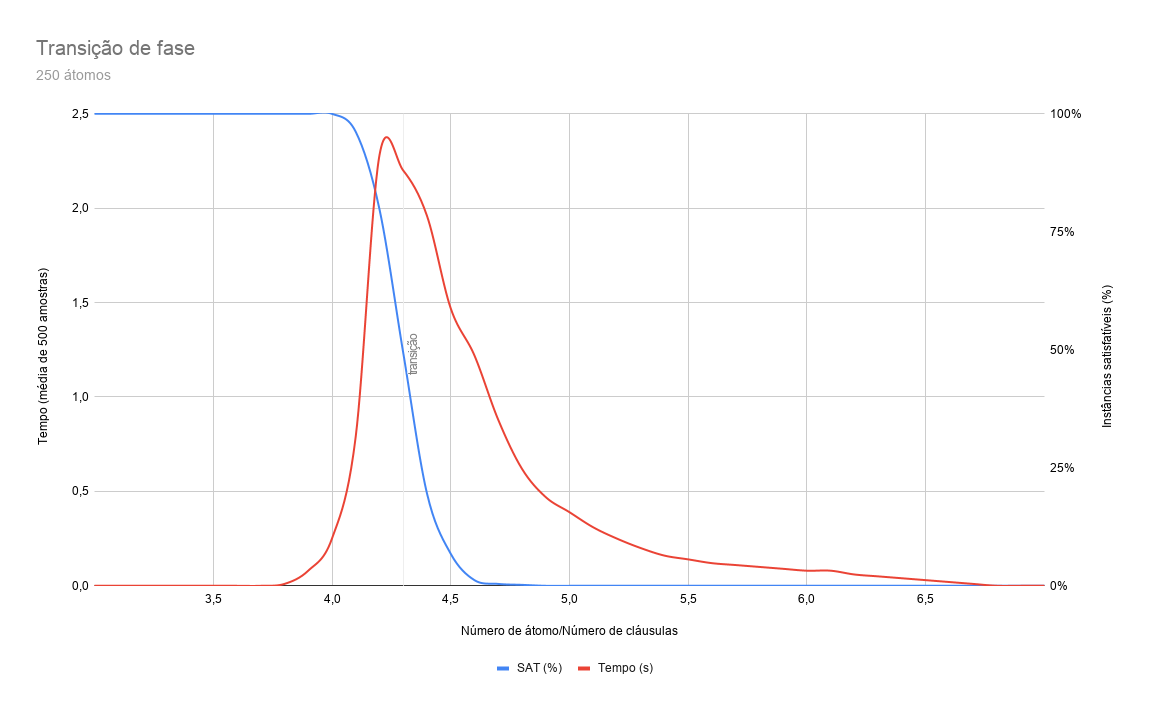
\includegraphics[width=\textwidth]{phase-transition.png}
  \caption{Transição de fase. A difículdade do problema 3-SAT ocorre no ponto em que há a mesma quatidade de instâncias satisfatíveis e insatisfatíveis.}
\end{figure}


\section{Relação entre as classes de complexidade de tempo}
\label{sec:hierarquia}

A discussão da seção anterior indica o pouco que conhecemos sobre a dificuldade de um problema.
A classe dos problemas NP-completos é a classe dos mais difíceis dentre os problemas NP.
Porém, não sabemos qual é relação entre a classe $P$ e a classe $NP$.
Acreditamos que essas classes sejam distintas, mas isso nunca foi provado.

A esta altura talvez seja interessante dar um passo atrás e nos perguntar uma coisa mais básica.
Conseguimos garantir que dado mais tempo somos capazes de resolver mais problemas?
A intuição que construímos no curso de Introdução à Analise de Algoritmo é de que sim.
Existem problemas para os quais existem solução quadrática, mas não existe solução linear.

O {\em Teorema da Hierarquia} foi possivelmente o primeiro resultado importante da teoria da complexidade.

\begin{theorem}{Hierarquia}
  \begin{displaymath}
    TIME(t(n)) \varsubsetneq TIME(O(t^3(n))
  \end{displaymath}
\end{theorem}
\begin{proof}
  A afirmação $TIME(t(n)) \subsetneq TIME(t(n) log^2(t(n)))$ é trivial.
  O que precisamos mostrar é que existe uma lingaguem que está em $TIME(t(n) log^2(t(n)))$, mas não está em $TIME(t(n))$.
  
  Vamos seguir um argumento de diagonalização similar ao da prova da indecidibilidade do problema da parada.
  Primeiro considere a seguinte linguagem:

  \begin{displaymath}
    H_t = \{ \langle M, \omega \rangle : \textrm{ M aceita $\omega$ em no máximo $t(|\omega|)$ passos }\}
  \end{displaymath}

  Para mostrar que lingaugem $H_t \in O(t^3(n))$ precisaríamos mostrar que é possível construir uma Máquina Universal de Turinal que simula $M$ em $O(t^3(n))$ passos.
  Essa é uma demonstração construtiva não muito interessante.
  Antes de passar para a próxima parte da demonstração, apenas comentaremos que é simples construir uma simulação de $M$ usando um MT com 3-fitas: uma que guarda a entrada $\omega$, uma que produz a saída e outra que processa a simulação é relativamente fácil de construir.
  Como vimos na Seção \ref{} é possível então transformar essa MT com 3-fitas em uma MT simples.
  Esse caminho resvole o problema em tempo proporcional a $O(t^3(n))$ que é suficiente para o que pretendemos mostrar a seguir.
  Cabe aqui comentar que é possível construir uma MT universal bem mais eficiente -- $O(t(n) log^2(t(n)))$ --, mas isso não é necessário para os resultados dessa seção.
  
  A parte interessante da demostração é provar que $H_t \notin TIME(t(\lfloor \frac{n}{2}\rfloor))$.
  Suponha por absurdo o contrário.
  Neste caso, seria possível construir a seguinte MT:

  \begin{displaymath}
    D_t(\langle M \rangle) =  \left\{\begin{array}{cl}
    \textrm{aceita} & \textrm{se $M_{H_t}$ não aceita $\langle M, M \rangle$}\\
    \textrm{rejeita} & \textrm{se $M_{H_t}$ aceita $\langle M, M \rangle$}\\ 
    \end{array}\right.
  \end{displaymath}

  Note que $D_t$ processa $langle M, M \rangle$ no mesmo tempo $t(\lfloor \frac{2n+1}{2}\rfloor) = t(n)$ que $M_{H_t}$.

  Podemos então repetir o mesmo argumento do problema da parada:
  O que ocorre se passarmos a descrição $\langle D_t \rangle$ como entrada para $D_t$?
  Se a entrada é aceita então $M_{H_t}$ não aceita $\langle D_t, D_t \rangle$, mas pela definião de $H_t$ isso significa que $D_t$ não aceita $\langle D_t \rangle$ o que é uma contradição.
  Se a entrada não é aceita então $M_{H_t}$ aceita $\langle D_t, D_t \rangle$ e também chegamos em uma contradição.
  Concluímos que $H_t \notin TIME(t(\lfloor \frac{n}{2}\rfloor))$.

  Juntando as duas partes existe um problema que não está em $TIME(t(n))$, mas está em $TIME(t(2n + 1)^3)$.
\end{proof}

Vamos introduzir agora mais uma classe de complexidade.
A classe $EXPTIME$ contém todos os problemas que podem ser decididos por uma Máquina de Turing determinísitica em tempo exponencial em relacão ao tamanho da entrada.
O teorema da hierarquia nos mostra que essa classe está propriamente contida na classe $P$

\begin{corollary}
  \begin{displaymath}
    P \subsetneq EXPTIME
  \end{displaymath}
\end{corollary}
\begin{proof}
  Partimos do fato conhecido que $P \subseteq TIME(2^n)$, ou seja, qualquer polinômio eventualemente se torna menor do que $2^n$.
  Mas pelo Teorema da Hierarquia temos que $TIME(2^n) \varsubsetneq TIME(2^{O(n^3)}) \subseteq EXPTIME$.
  Portanto, $P \varsubsetneq EXPTIME$.
\end{proof}

Vamos resumir o que sabemos até agora sobre as classes de complexidade.
Apresentamos quatro classes:
\begin{enumerate}
\item $P$: a classe dos problemas decidíveis em tempo polinomial por uma MT determinística.
\item $NP$: a classe dos problemas que possuem certificado polinomial.
\item $coNP$: a classe dos problemas que possuem desqualificador polinomial.
\item $EXPTIME$: a classe dos problemas decidívei e tempo exponencial por um MT determinística.
\end{enumerate}

Sabemos que $P \subseteq NP$ e que $P \subseteq coNP$.
Além disso, quando introduzimos as MT não determinísticas, vimos que é possível simular qualquer uma delas em uma MT determinística.
Essa simulação toma tempo exponencial e, portanto, $NP \subseteq EXPTIME$.
Não é difícil perceber que da mesma forma temos que $coNP \subseteq EXPTIME$.
Por fim, acabamos de demonstrar que $P \neq EXPTIME$.
Sabemos, portanto que existem problemas que podemos resolver em tempo exponencial, mas que não são resolvíveis em tempo polinomial.
Não sabemos, de fato esse é o maior problemas em aberto na computação (!), se $P \neq NP$.
Na verdade não sabemos praticamente mais nada sobre as relações entre essas classes do que foi aqui exposto.

%\section{Complexidade de Espaço}
%\label{sec:espaco}

% definição de PSPACE e NPSACE
% Teorema de Salvitch
